% This is the main beamer template file.

\documentclass[10pt]{beamer} % normal 4:3 aspect ratio
% \documentclass[aspectratio=169,10pt]{beamer}  % widescreen 16:9 aspect ratio
\usetheme{default}
\usepackage{graphicx}
\usepackage{multicol}

% Set your font here
\usefonttheme{professionalfonts} % using non standard fonts for beamer
\usefonttheme{serif} % default family is serif
\usepackage{fontspec}
\setmainfont{Palatino}

\setbeamertemplate{navigation symbols}{} % Turn off the navigation symbols
\setbeamerfont{frametitle}{size=\fontsize{12pt}{8pt}}
\setbeamertemplate{footline}[frame number]

% \setbeamersize{text margin left=0mm, text margin right=0mm}


% --- the presentation begins here ----------------%
%\AtBeginSection[]
%{
%   \begin{frame}
%   \frametitle{}
%   \tableofcontents[currentsubsection, 
%       hideothersubsections, 
%       sectionstyle=show/shaded, 
%       subsectionstyle=show/shaded, 
%]
%   \end{frame}
%}

\title{My awesome presentation $|\eta_{1,2,3}|$}
\subtitle{My awesome subtitle}
\author[My collaboration]{My collaboration}
\date{\today}


\begin{document}

%--- the titlepage frame -------------------------%
%  use [fragile] to get verbatim text to work
\begin{frame}
  \titlepage
\end{frame}

\begin{frame}{Table of Contents}
    \begin{multicols}{2}
        \tableofcontents
    \end{multicols}
\end{frame}

%  Plot ALL the things

\section{A 4 plot slide}
\begin{frame}{A 4 plot slide}
Some top text
\begin{columns}
\begin{column}{0.4\textwidth}
\begin{center}
Optional title
\\
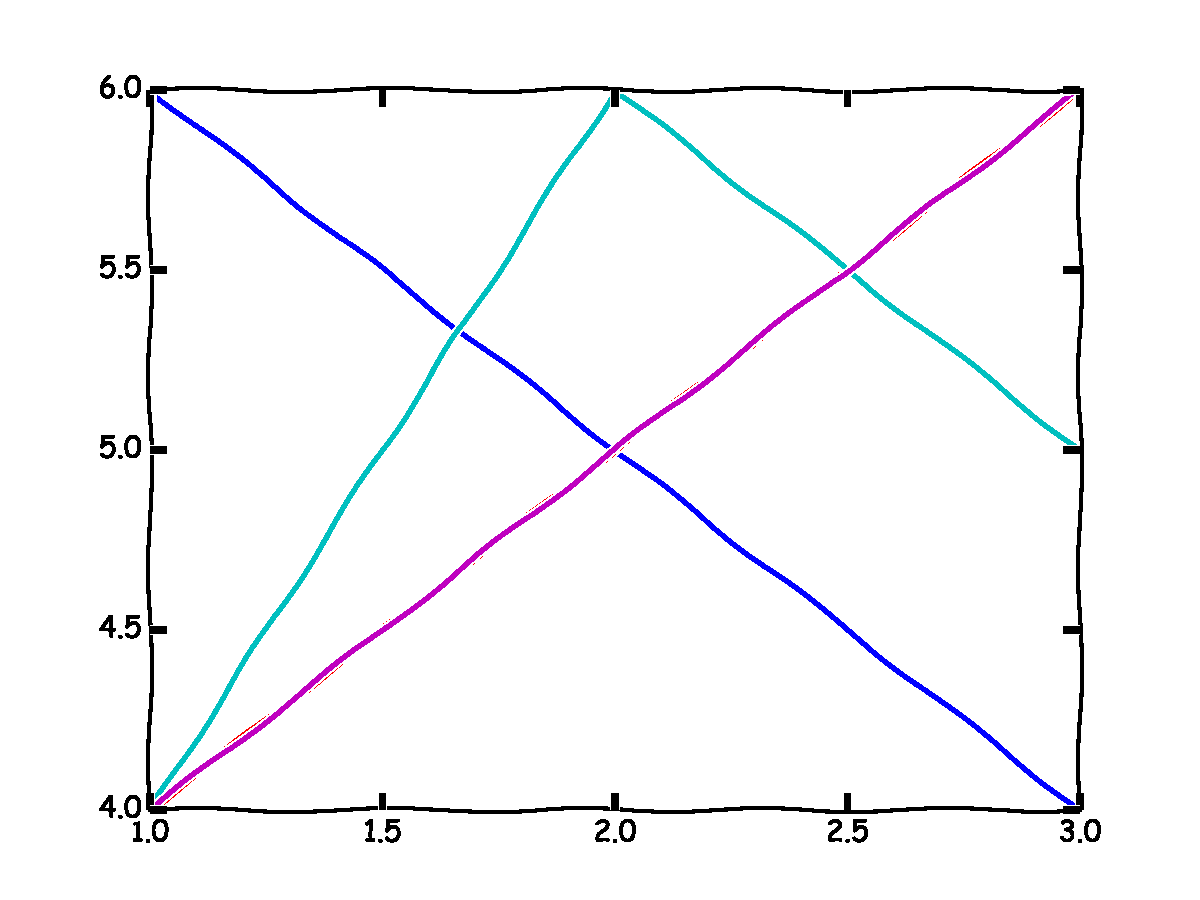
\includegraphics[width=\textwidth]{example/plot1.pdf}
\\
Plot 3 title
\\
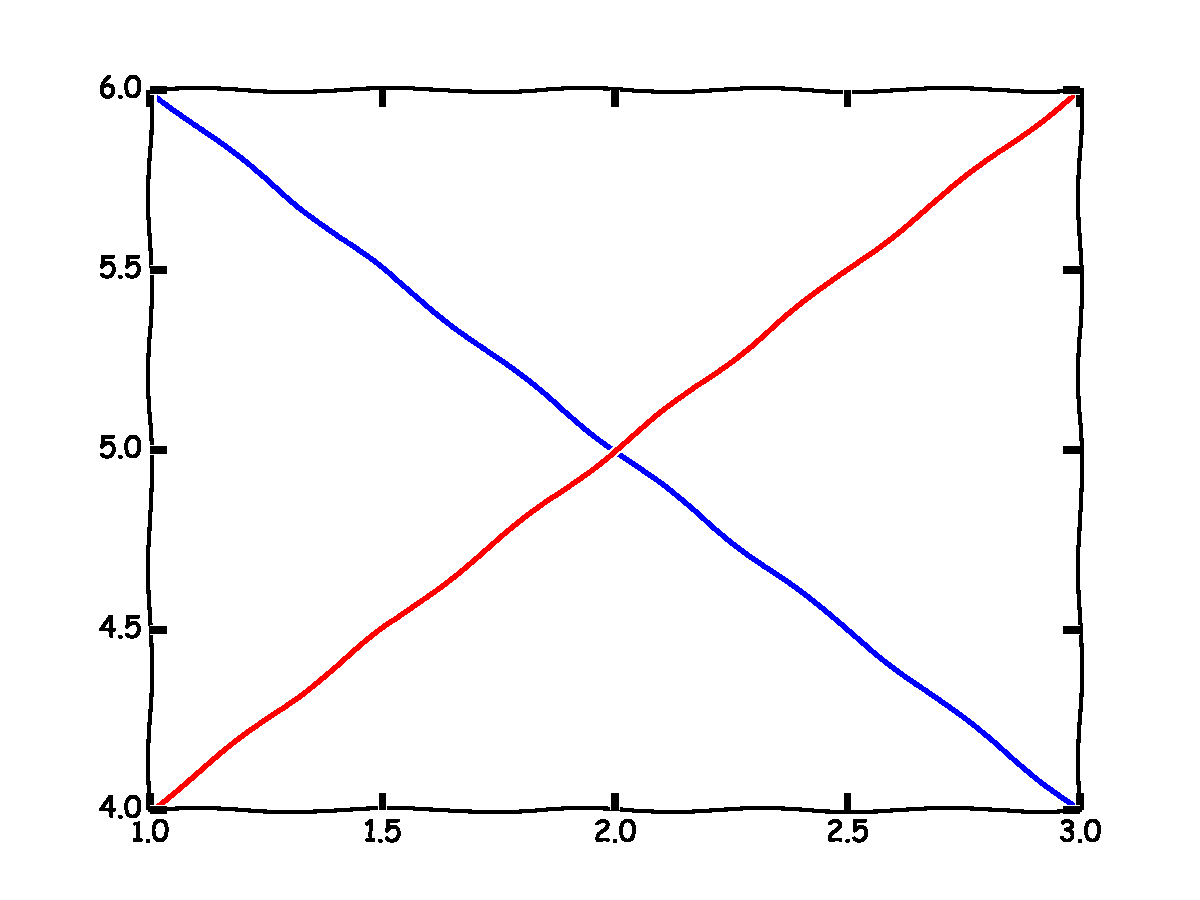
\includegraphics[width=\textwidth]{example/plot3.pdf}
\\
\end{center}
\end{column}

\begin{column}{0.4\textwidth}
\begin{center}
Plot 2 title
\\
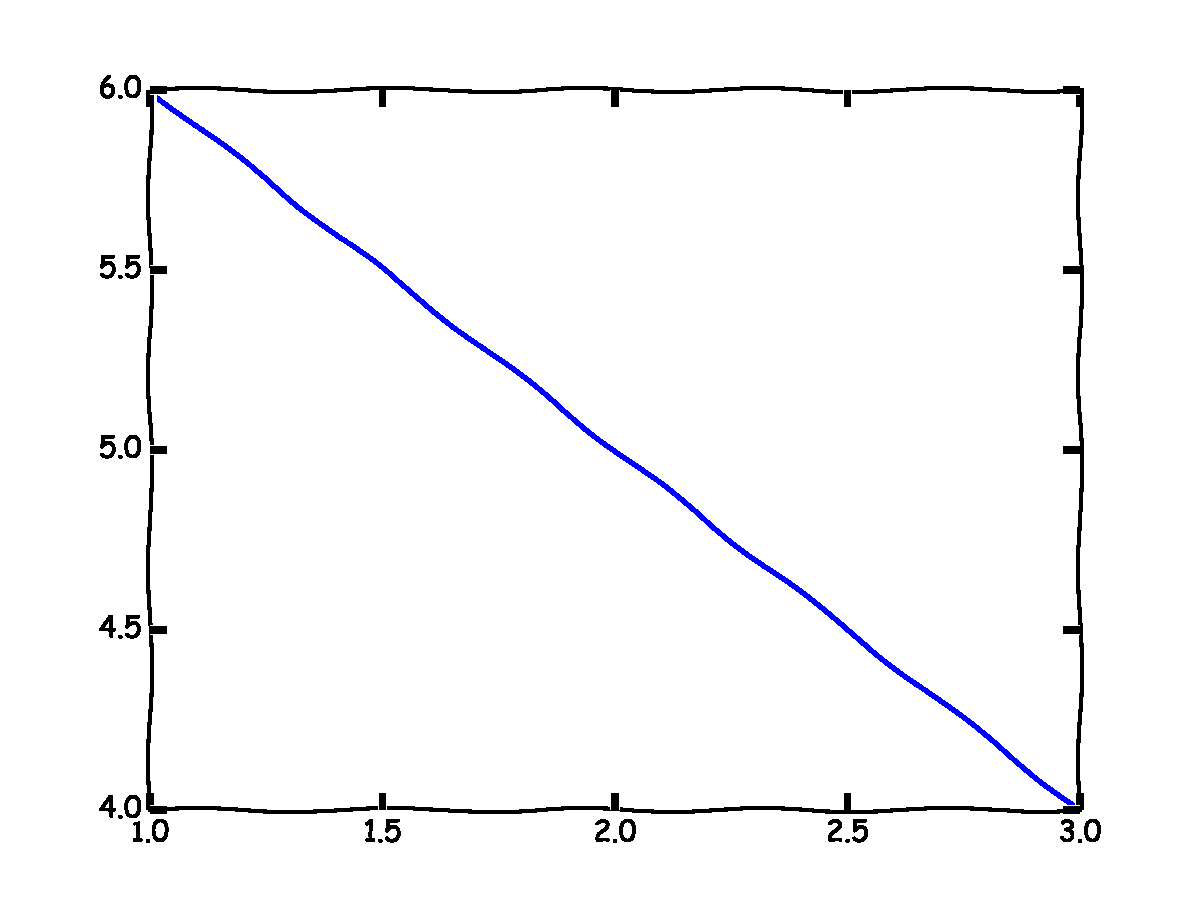
\includegraphics[width=\textwidth]{example/plot2.pdf}
\\
Plot 4 title
\\
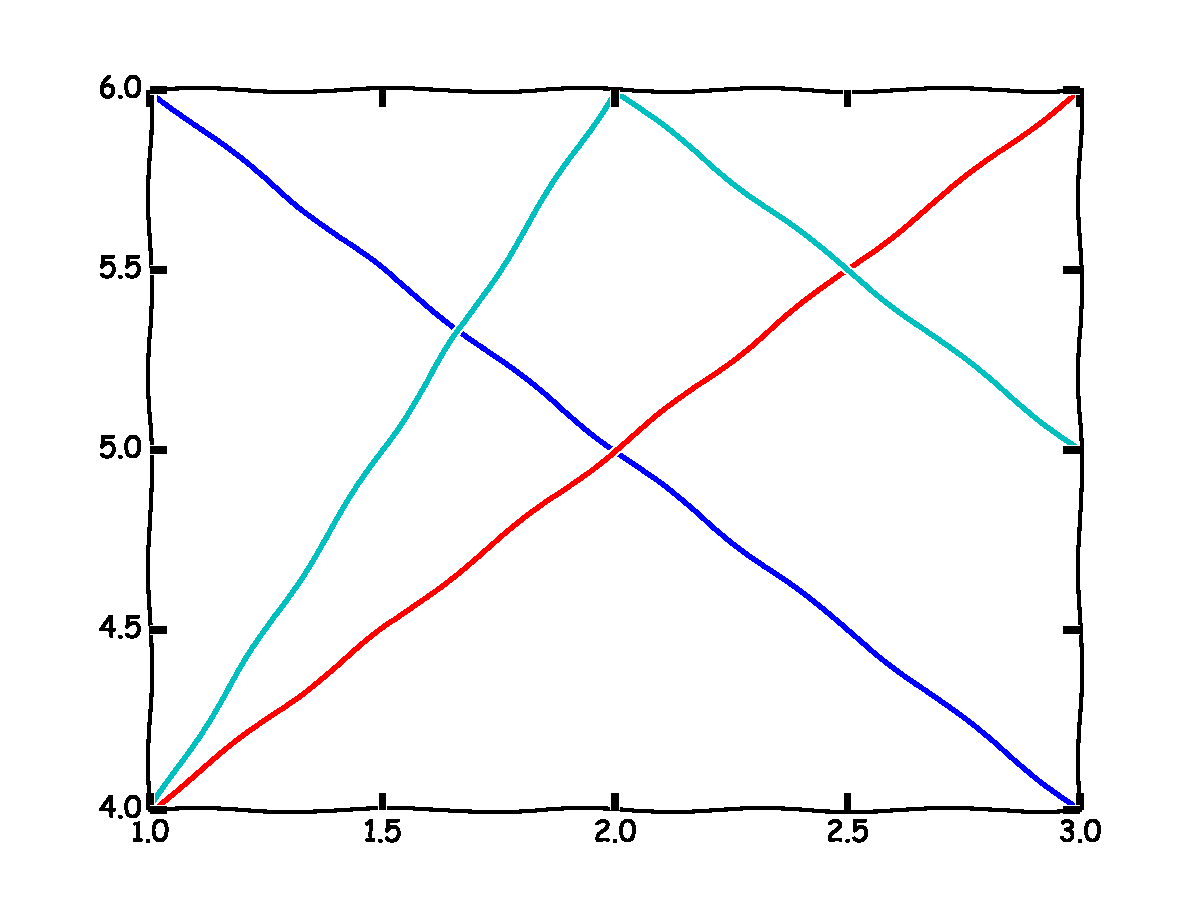
\includegraphics[width=\textwidth]{example/plot4.pdf}
\\
\end{center}
\end{column}
\end{columns}
Some bottom text
\end{frame}

\section{Two plot slide}
\begin{frame}{Two plot slide}
With no plot titles
\begin{columns}
\begin{column}{0.5\textwidth}
\begin{center}
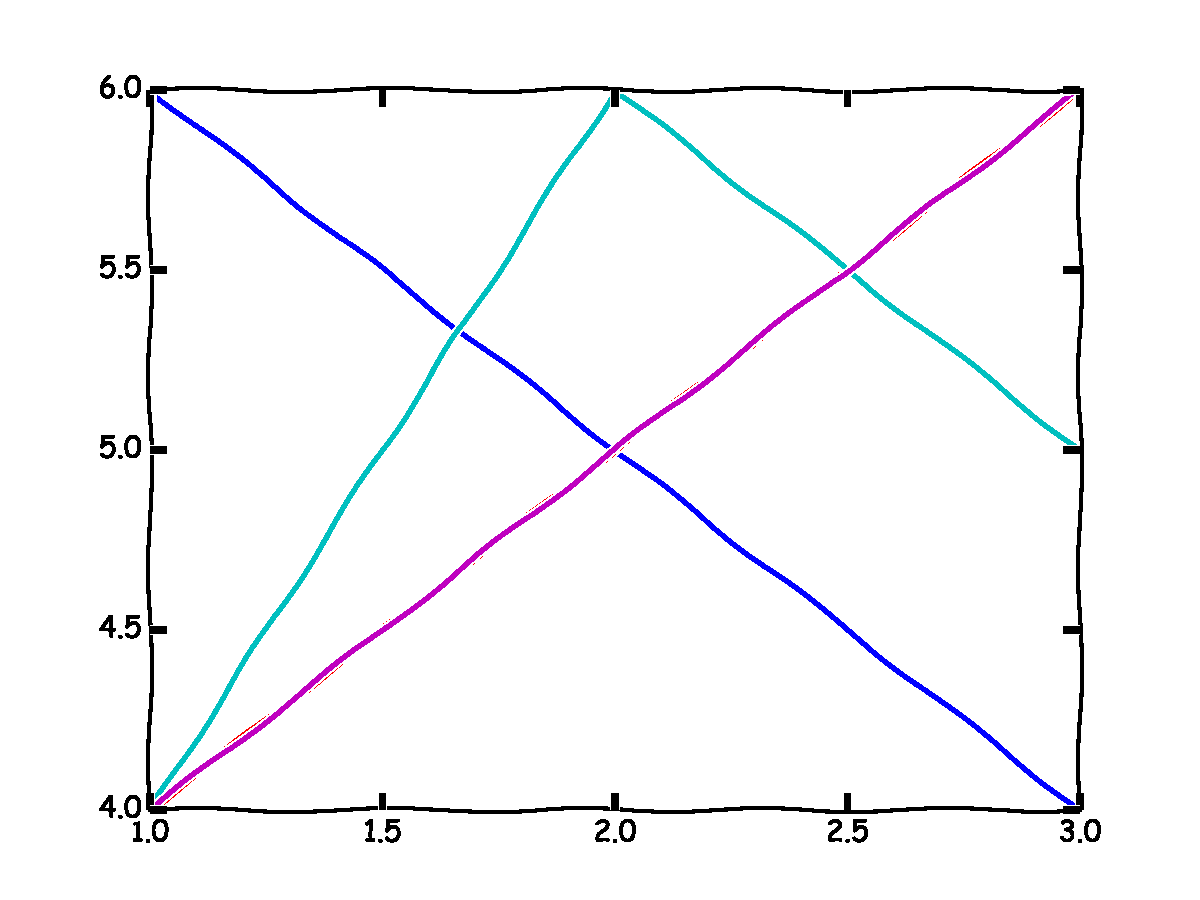
\includegraphics[width=\textwidth]{example/plot1.pdf}
\\
\end{center}
\end{column}

\begin{column}{0.5\textwidth}
\begin{center}
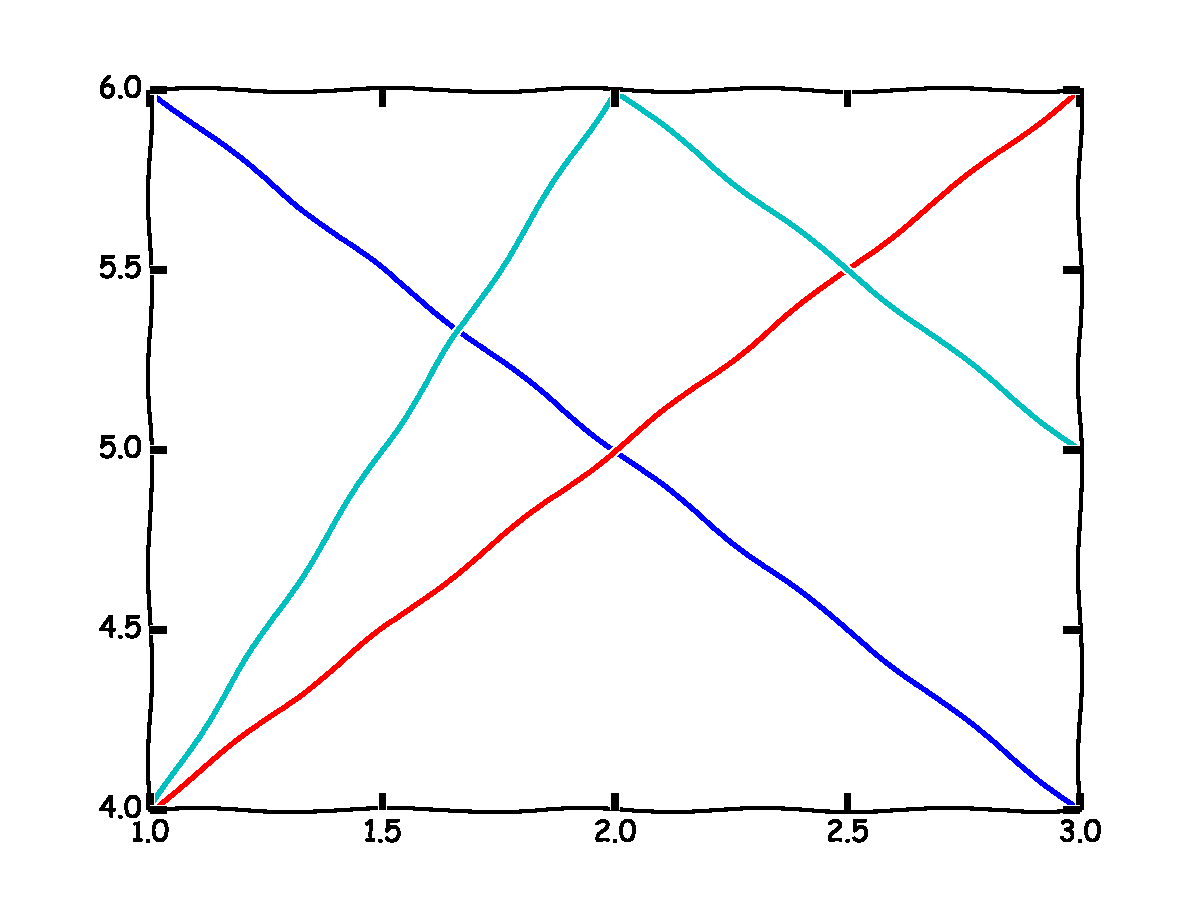
\includegraphics[width=\textwidth]{example/plot4.pdf}
\end{center}
\end{column}
\end{columns}
blah blah blah
\end{frame}

\section{Simple one plot slide}
\begin{frame}{Simple one plot slide}
Some top text
\begin{center}
Optional title
\\
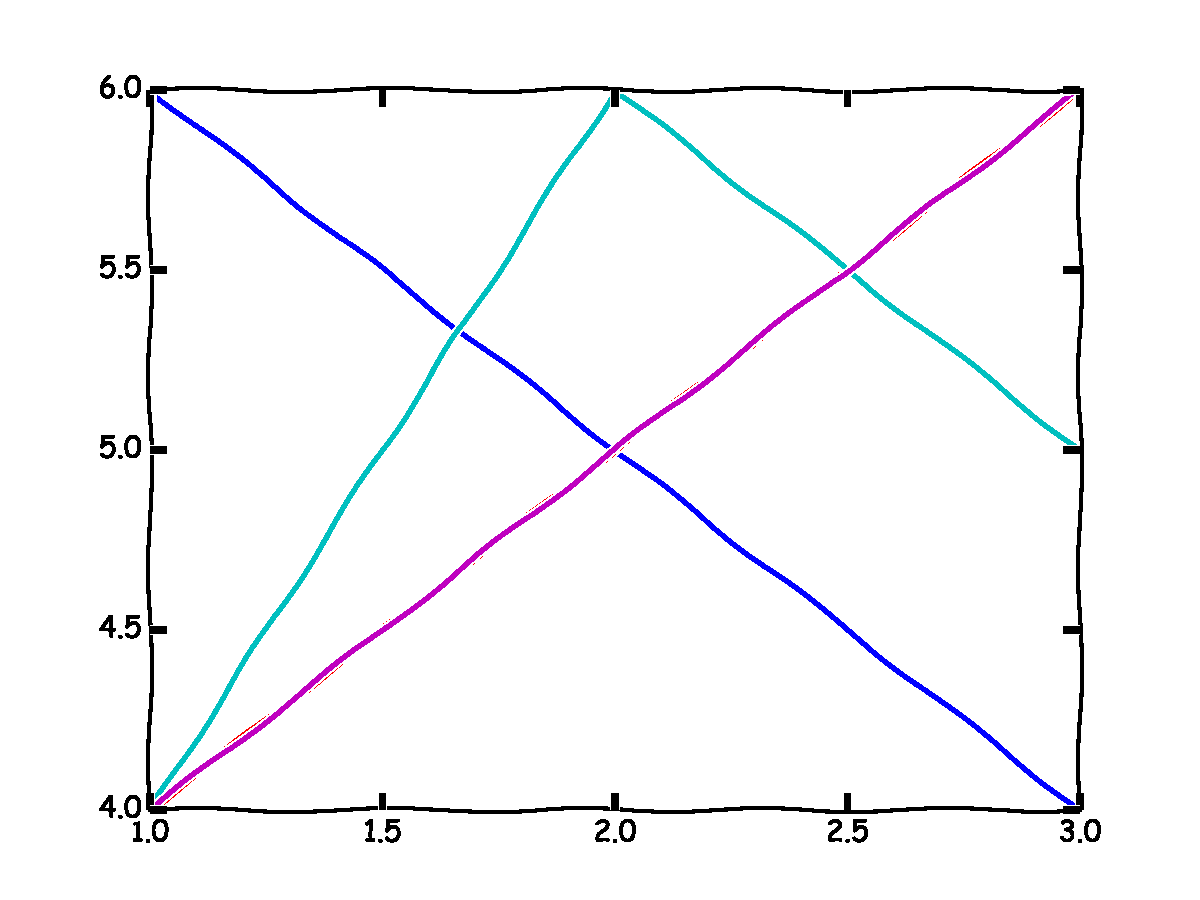
\includegraphics[width=0.8\textwidth]{example/plot1.pdf}
\\
\end{center}
Some bottom text
\end{frame}

\section{A whopping 6 plots}
\begin{frame}{A whopping 6 plots}
Are you crazy
\begin{columns}
\begin{column}{0.33\textwidth}
\begin{center}
Optional title
\\
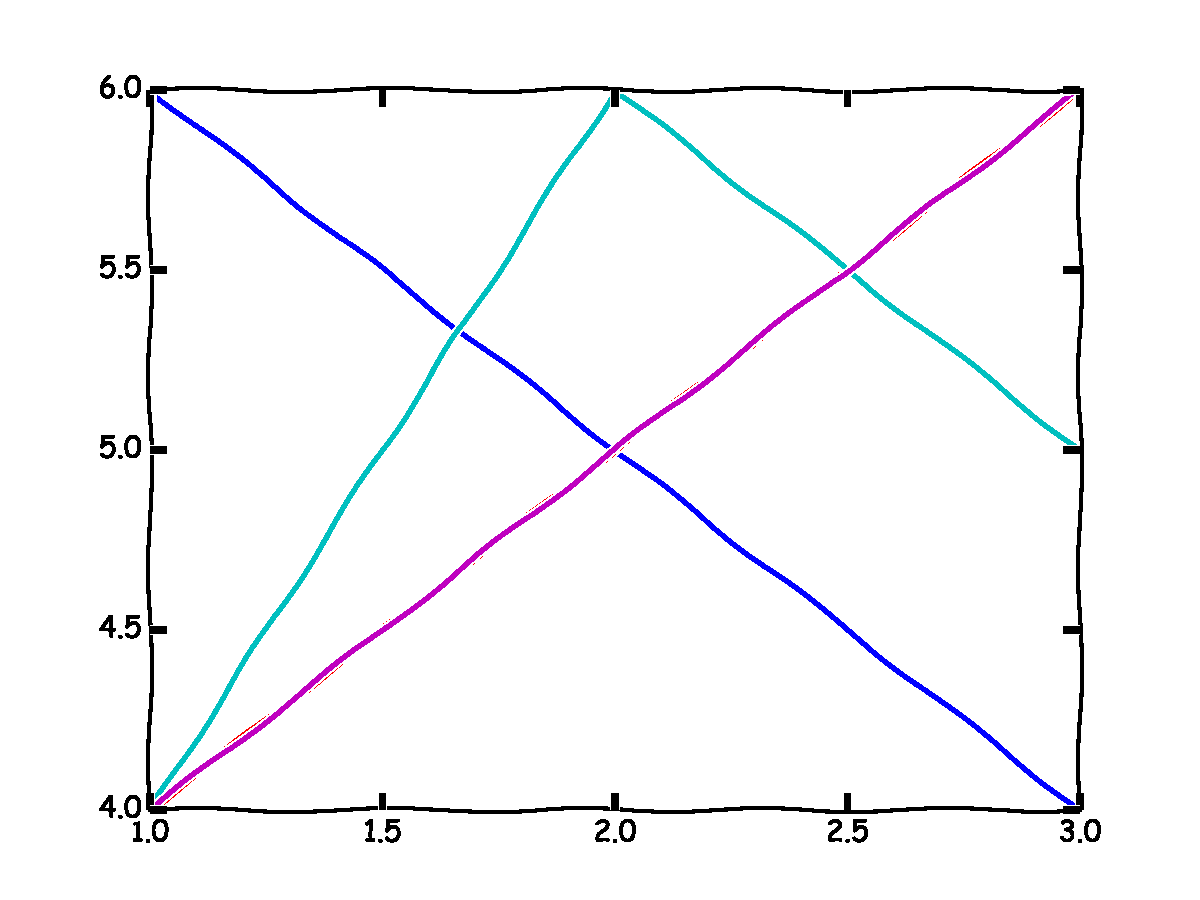
\includegraphics[width=\textwidth]{example/plot1.pdf}
\\
Plot 4 title
\\
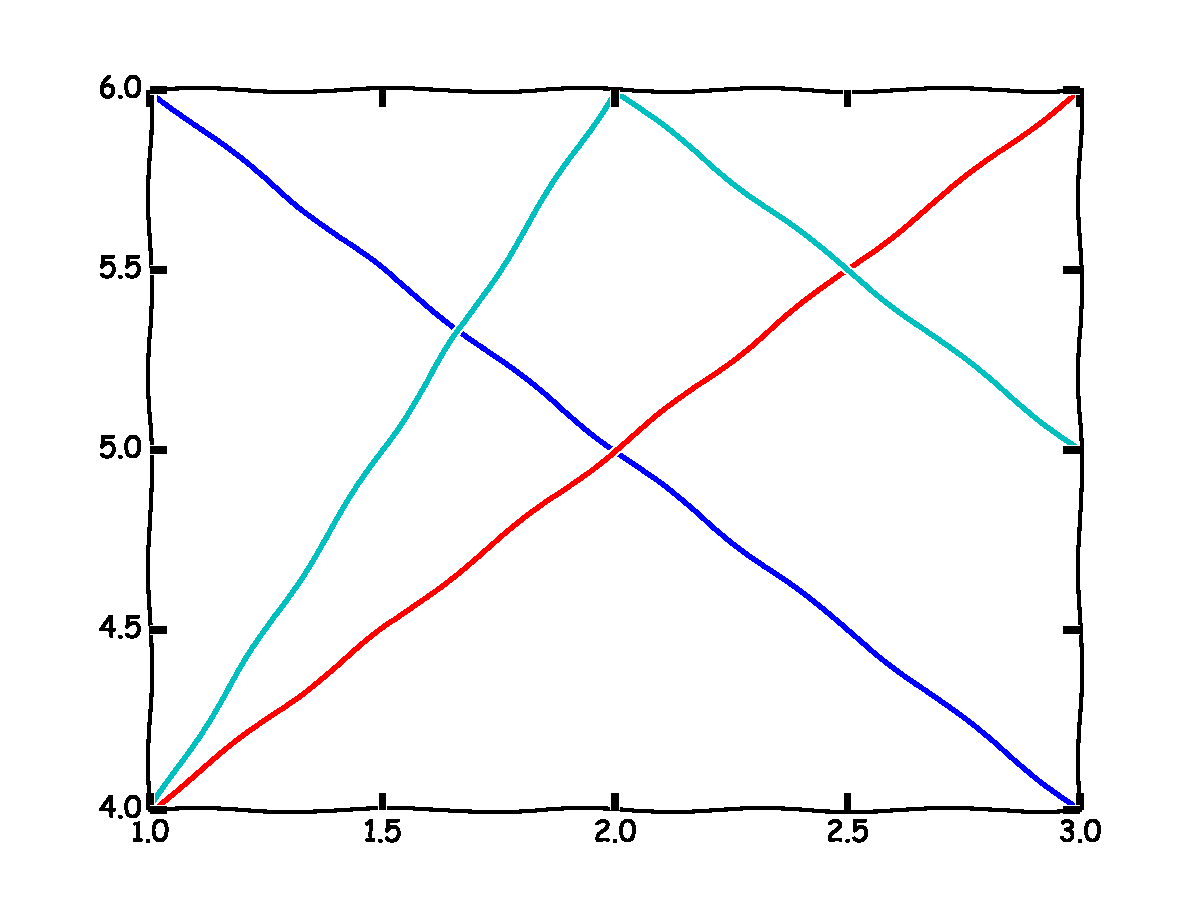
\includegraphics[width=\textwidth]{example/plot4.pdf}
\end{center}
\end{column}

\begin{column}{0.33\textwidth}
\begin{center}
Plot 2 title
\\
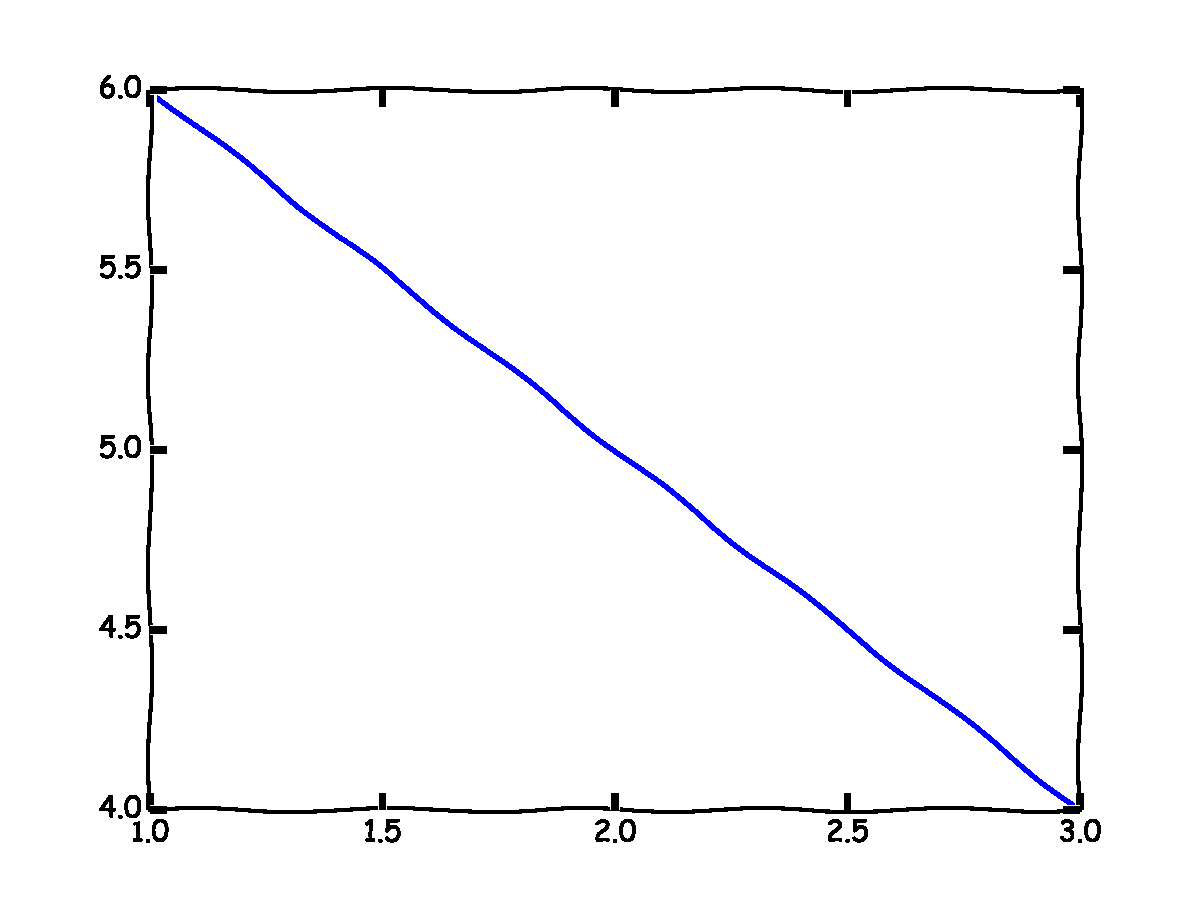
\includegraphics[width=\textwidth]{example/plot2.pdf}
\\
Plot 5 title
\\
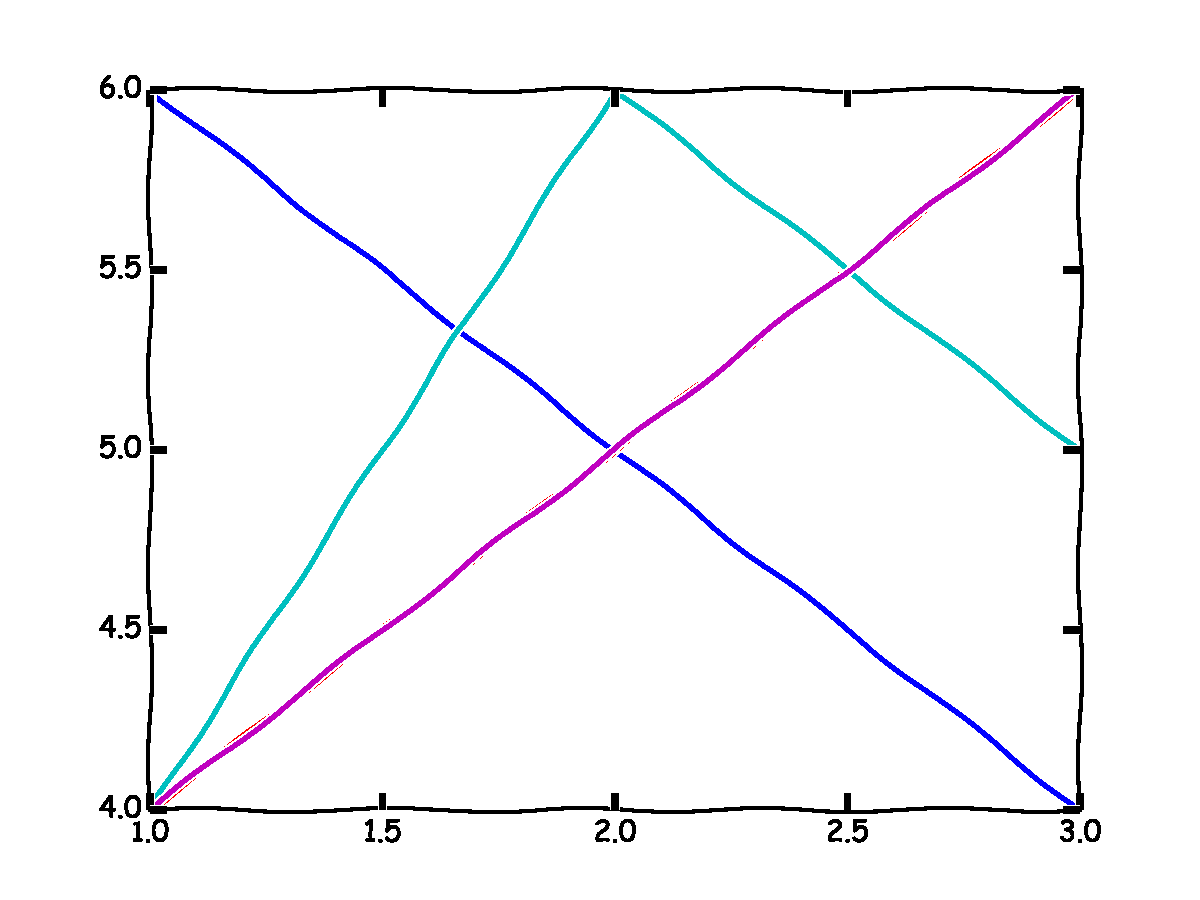
\includegraphics[width=\textwidth]{example/plot1.pdf}
\end{center}
\end{column}

\begin{column}{0.33\textwidth}
\begin{center}
Plot 3 title
\\
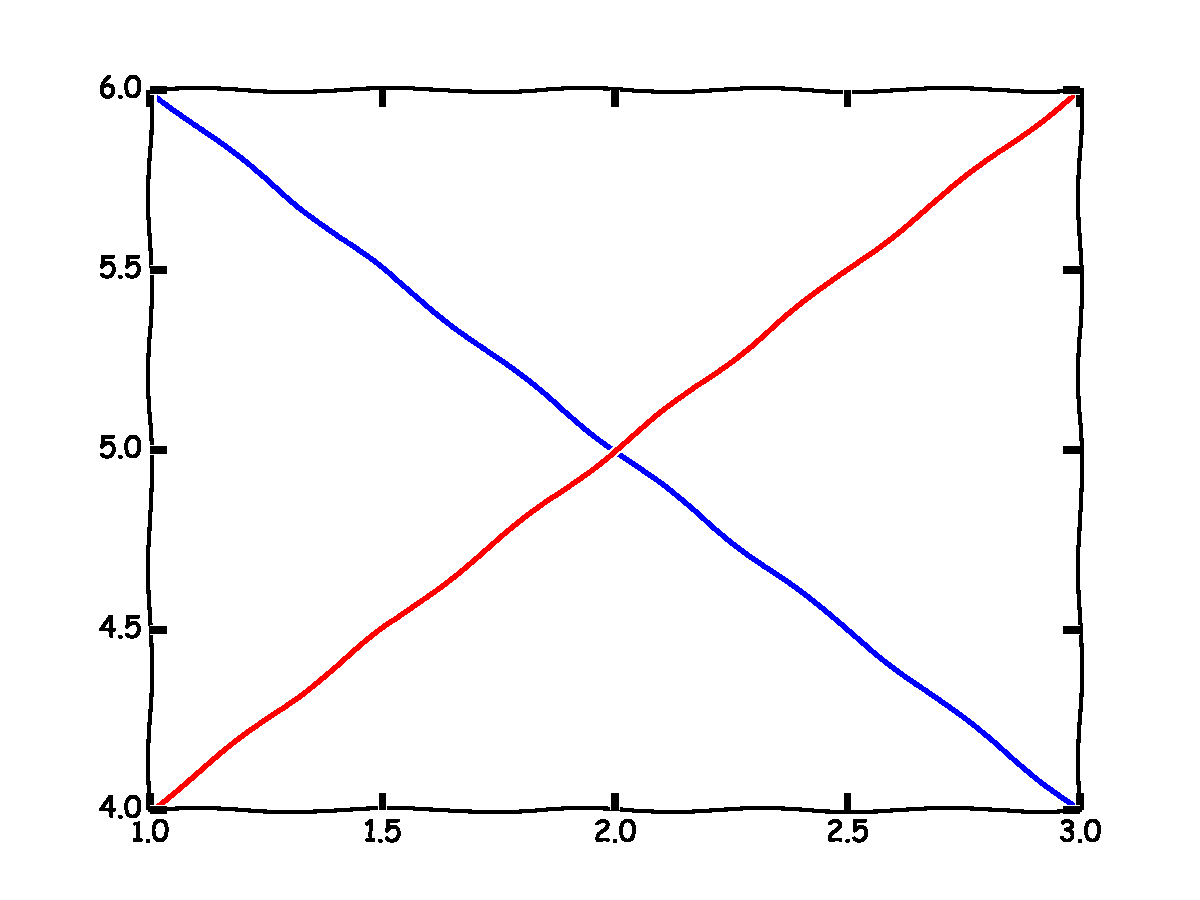
\includegraphics[width=\textwidth]{example/plot3.pdf}
\\
Plot 6 title
\\
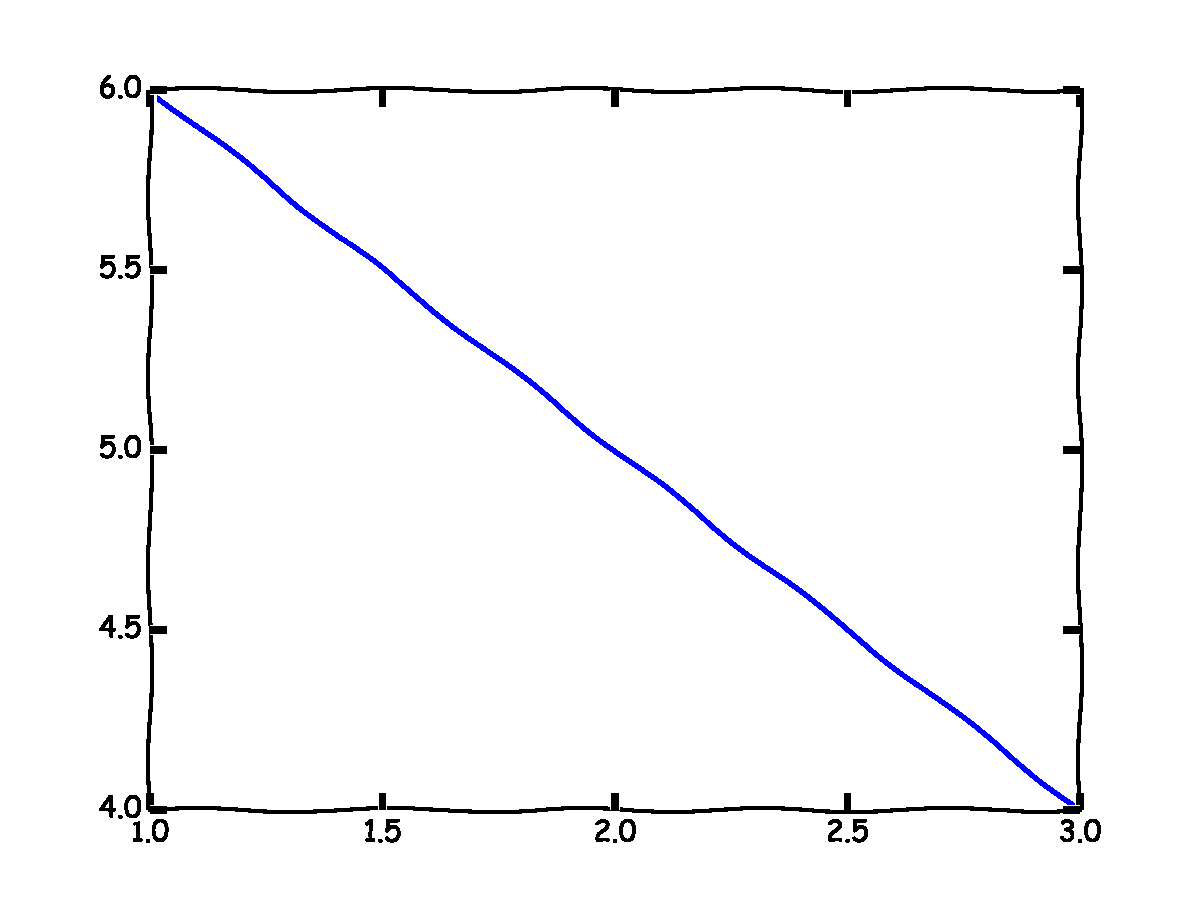
\includegraphics[width=\textwidth]{example/plot2.pdf}
\end{center}
\end{column}
\end{columns}
Some bottom text
\end{frame}


\end{document}